\documentclass[11pt]{article}

\usepackage{amsmath}
\usepackage{amsthm}
\usepackage[spanish]{babel}
\usepackage{amssymb}
\usepackage{mathtools}
\usepackage{multirow}
\usepackage{colortbl}
\usepackage{color}
\usepackage{multicol}
\usepackage{float}
\usepackage{biblatex}
\providecommand{\N}{\mathbb{N}}
\providecommand{\Z}{\mathbb{Z}}
\providecommand{\Q}{\mathbb{Q}}
\providecommand{\R}{\mathbb{R}}
\providecommand{\C}{\mathbb{C}}
\providecommand{\H}{\mathcal{H}}
\providecommand{\Im}[1]{Im(#1)}
\providecommand{\Re}[1]{Re(#1)}
\providecommand{\conjugate}[1]{\bar{#1}}
\providecommand{\pescalar}[2]{\langle #1,#2 \rangle}
\providecommand{\braket}[2]{\left\langle#1\mid#2\right\rangle}
\providecommand{\bra}[1]{\left\langle#1\right\rvert}
\providecommand{\ket}[1]{\left\lvert#1\right\rangle}
\providecommand{\ketbra}[2]{\left\lvert#1\right\rangle\!\left\langle#2\right\rvert}
\providecommand{\avg}[1]{\left\langle#1\right\rangle}
\providecommand{\abs}[1]{\lvert#1\rvert}
\providecommand{\nor}[1]{\lVert#1\rVert}
\providecommand{\operatoravg}[3]{\left\langle#1|#2|#3\right\rangle}
\providecommand{\set}[1]{\left\{#1\right\}}
\providecommand{\so}{\Rightarrow}
\providecommand{\tq}{\mid}
\providecommand{\where}{\mathrel{}\middle|\mathrel{}}

\definecolor{unir-azul-flojo}{RGB}{230,244,249}
\definecolor{unir-azul-fuerte}{RGB}{0,152,205}
%Kets notables
\newcommand{\ketMas}{\frac{1}{\sqrt{2}}(\ket{0}+\ket{1})}
\newcommand{\ketMenos}{\frac{1}{\sqrt{2}}(\ket{0}-\ket{1})}
\newcommand{\ketIMas}{\frac{1}{\sqrt{2}}(\ket{0}+i\ket{1})}
\newcommand{\ketIMenos}{\frac{1}{\sqrt{2}}(\ket{0}-i\ket{1})}
\newcommand{\ketBellUno}{\frac{1}{\sqrt{2}}(\ket{00}+\ket{11})}
\newcommand{\ketBellDos}{\frac{1}{\sqrt{2}}(\ket{00}-\ket{11})}
\newcommand{\ketBellTres}{\frac{1}{\sqrt{2}}(\ket{10}+\ket{01})}
\newcommand{\ketBellCuatro}{\frac{1}{\sqrt{2}}(\ket{10}-\ket{01})}

%OPERADORES 2x2
\newcommand{\matrixX}{\begin{pmatrix}0 & 1 \\ 1 & 0\end{pmatrix}}
\newcommand{\matrixY}{\begin{pmatrix}0 & -i \\ i & 0\end{pmatrix}}
\newcommand{\matrixZ}{\begin{pmatrix}1 & 0 \\ 0 & -1\end{pmatrix}}
\newcommand{\matrixH}{\frac{1}{\sqrt {2}}  \begin{pmatrix}1 & 1 \\ 1 & -1\end{pmatrix}}
%OPERADORES 4x4
\newcommand{\matrixCNOT}{\begin{pmatrix}1 & 0 & 0 & 0 \\ 0 & 0 & 0 & 1 \\ 0 & 0 & 1 & 0 \\ 0 & 1 & 0 & 0\end{pmatrix}}
\usepackage[left=1.75cm,
	right=1.5cm,
	top=3.52cm,
	bottom=3.23cm]{geometry}
\usepackage{fancyhdr}
\usepackage{graphicx}
\usepackage{sectsty}
\setlength{\parskip}{\baselineskip}
\newcommand{\personalheader}[2]{
	\pagestyle{fancy}
  \setlength{\headheight}{70.866141732pt}
  \setlength{\topmargin}{-50pt}
  \setlength{\headsep}{0pt}
  \setlength{\footskip}{13.866141732pt}
	\renewcommand{\headrulewidth}{0pt}
	\fancyhead[R]{#1\\\ \\#2}
	\fancyfoot{}
	\fancyfoot[R]{\thepage}
}
\newcommand{\titulo}[1]{\textcolor{unir-azul-fuerte}{\LARGE{\textbf{#1}}}\vspace{0.1in}}
\newcommand{\primersubtitulo}[1]{\textcolor{unir-azul-fuerte}{\large #1}}
\newcommand{\subtitulo}[1]{\vspace{0.1in}\textcolor{unir-azul-fuerte}{\large #1}}
\newcommand{\seccion}[1]{\vspace{0.1in}\textbf{#1}}
\renewcommand{\labelitemi}{$\textcolor{unir-azul-fuerte}{\bullet}$}
\renewcommand{\labelitemii}{$\textcolor{unir-azul-fuerte}{\cdot}$}
\renewcommand{\labelitemiii}{$\textcolor{unir-azul-fuerte}{\diamond}$}
\renewcommand{\labelitemiv}{$\textcolor{unir-azul-fuerte}{\ast}$}
\sectionfont{\color{unir-azul-fuerte}}
\subsectionfont{\color{unir-azul-fuerte}}
\subsubsectionfont{\color{unir-azul-fuerte}}
\renewcommand*\contentsname{\textcolor{unir-azul-fuerte}{Índice de contenidos}}
\renewcommand{\listfigurename}{\textcolor{unir-azul-fuerte}{Índice de figuras}}
\renewcommand{\listtablename}{\textcolor{unir-azul-fuerte}{Índice de tablas}}
\begin{document}
	\personalheader{Nombre y apellidos del estudiante}{Título del Trabajo Fin de Estudios}
	\begin{center}
	
\includegraphics[width=10.6cm,height=2.88cm]{logo}

	\Huge Universidad Internacional de La Rioja

	\huge Escuela Superior de Ingeniería y \\ Tecnología

	\vspace{100pt}

	\LARGE Máster Universitario en Computación Cuántica

	\Huge \textcolor{unir-azul-fuerte}{Título del Trabajo Fin de Estudios}
	\normalsize

	\vspace{100pt}

\end{center}
\begin{tabular}{ll}
	Trabajo fin de estudio presentado por: & \\
	Tipo de trabajo:                       & \\
	Director/a:                            & \\
	Fecha:                                 & \\
\end{tabular}
\newpage
	\titulo{Resumen}

En este apartado se introducirá un breve resumen en español del trabajo realizado. Este resumen debe incluir el objetivo o propósito de la investigación, la metodología, los resultados y las conclusiones.

(Aproximadamente 150 palabras)

\textbf{Palabras clave:} (De 3 a 5 palabras)
	\chapter{Abstract}

En este apartado se introducirá un breve resumen en español del trabajo realizado (extensión máxima: 150 palabras). Este resumen debe incluir el objetivo o propósito de la investigación, la metodología, los resultados y las conclusiones.

{\bf Keywords:} Se deben incluir de 3 a 5 palabras claves en inglés
	\tableofcontents
\newpage
	\listoffigures
	\listoftables

	\chapter{Introducción}

El primer capítulo es siempre una introducción. En ella debes resumir de forma esquemática pero suficientemente clara lo esencial de cada una de las partes del Trabajo. La lectura de este primer capítulo ha de dar una primera idea clara de lo que se pretendía, las conclusiones a las que se ha llegado y del procedimiento seguido.

Como tal, es uno de los capítulos más importantes de la memoria. Las ideas principales a transmitir son la identificación del problema a tratar, la justificación de su importancia, los objetivos generales (a grandes rasgos) y un adelanto de la contribución que esperas hacer.

Típicamente una introducción tiene tres apartados: Motivación, Planteamiento del trabajo, Estructura del trabajo. (Texto Normal del menú de estilos.)

(Ejemplo de nota al pie\footnote{Ejemplo de nota al pie.}.)

\section{Motivación/justificación del tema a tratar}

¿Cuál es el problema que quieres tratar?

¿Cuáles crees que son las causas?

¿Por qué es relevante el problema?

A continuación, se indica con un ejemplo cómo deben introducirse los títulos y las fuentes en tablas y figuras.

\begin{table}[t]
	\begin{center}
	\caption{Ejemplo de tabla con sus principales elementos.}
	\label{tab:tab-1}
	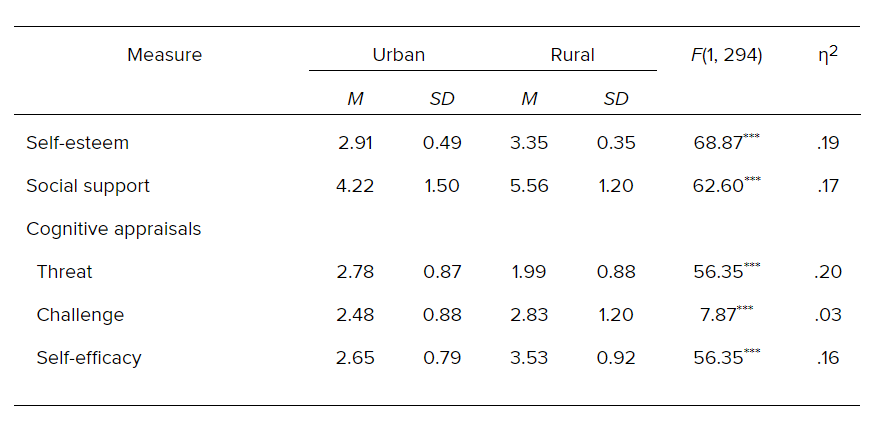
\includegraphics[width=4.90737in,height=2.42708in]{tabla}

	\small Fuente: American Psychological Association, 2020e.
	\end{center}
\end{table}

\begin{figure}[ht]
	\begin{center}
		\caption{Ejemplo de figura realizada para nuestro Trabajo.}
		\label{fig:fig-1}
		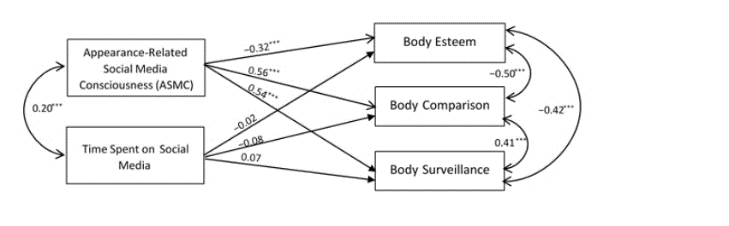
\includegraphics[width=4.90737in,height=2.42708in]{figura}

		\small Fuente: American Psychological Association, 2020f.
	\end{center}
\end{figure}

\section{Planteamiento del problema}

¿Cómo se podría solucionar el problema?

¿Qué es lo que se propone?

Aquí describes tu objetivo en términos generales.

\section{Estructura del Trabajo}

Aquí describes brevemente lo que vas a contar en cada uno de los capítulos siguientes.
	\section{Contexto y estado del arte}

Después de la introducción, se suele describir el contexto de aplicación. Suele ser un capítulo (o dos en ciertos casos) en el que se estudia a fondo el dominio de aplicación, citando numerosas referencias. Debe aportar un buen resumen del conocimiento que ya existe en el campo de los problemas habituales identificados.

Es conveniente que revises los estudios actuales publicados en la línea elegida, y deberás consultar diferentes fuentes. No es suficiente con la consulta on-line, es necesario acudir a la biblioteca y consultar manuales técnicos.

Hay que tener presente los autores de referencia en la temática del trabajo de investigación. Si se ha excluido a alguno de los relevantes hay que justificar adecuadamente su exclusión. Si por la extensión del trabajo no se puede señalar a todos los autores, habrá que justificar por qué se han elegido unos y se ha prescindido de otros.

La organización específica en secciones dependerá estrechamente el trabajo concreto que vayas a realizar. En este punto será fundamental la colaboración con tu DIRECTOR, él podrá asesorarte y guiarte, aunque siempre debes tener claro que el trabajo fundamental es tuyo.

El capítulo debería concluir con una última sección de resumen de conclusiones, resumiendo las principales averiguaciones del estudio del dominio y cómo van a afectar al desarrollo específico del trabajo.

Recuerda que para citar trabajos de diferentes autores es fundamental e imprescindible seguir el formato APA, según se describe en el documento Normativa_APA.pdf disponible en el apartado de Documentación del Aula de información general del Máster Universitario en Computación Cuántica (MUCC). No se debe mencionar, ni utilizar ninguna fuente, sin citarla apropiadamente.

\subsection{Objetivos y metodología de trabajo}

Este tercer capítulo es el puente entre el estudio del dominio y la contribución a realizar. Según el trabajo concreto, el bloque se puede organizar de distintas formas, pero hay tres elementos que deben estar presentes con mayor o menor detalle: (1) objetivo general, (2) objetivos específicos y (3) metodología de trabajo.

Es muy importante, por no decir imprescindible, que los objetivos (general y específicos) sean SMART (Doran, 1981) según la idea de George T. Doran que utilizó la palabra smart (inteligente en inglés) para definir las características de un objetivo:
\begin{itemize}
	\item[S] Specific / Específico: que exprese claramente qué es exactamente lo que se quiere conseguir.
	\item[M] Measurable / Medible: que se puedan establecer medidas que determinen el éxito o fracaso y también el progreso en la consecución del objetivo.
	\item[A] Attainable / Alcanzable: que sea viable su consecución en base al esfuerzo, tiempo y recursos disponibles para conseguirlo.
	\item[R] Relevant / Relevante: que tenga un impacto demostrable, es decir que sea útil para un propósito concreto.
	\item[T] Time-Related / Con un tiempo determinado: que se pueda llevar a cabo en una fecha determinada.
\end{itemize}

\subsubsection{Objetivo general}

Los trabajos aplicados se centran en conseguir un impacto concreto, demostrando la efectividad de una tecnología, proponiendo una nueva metodología o aportando nuevas herramientas tecnológicas. El objetivo por tanto no debe ser sin más “crear una herramienta” o “proponer una metodología”, sino que debe centrarse en conseguir un efecto observable. Además, como se ha dicho antes el objetivo general debe ser SMART.

Ejemplo de objetivo general SMART: Mejorar el servicio de audio guía de un museo convirtiéndolo en una guía interactiva controlada por voz y valorada positivamente, un mínimo 4 sobre 5, por los visitantes del museo.

Este objetivo descrito anteriormente podría dar lugar a un trabajo de tipo 2 (desarrollo de software) que plantease el desarrollo de un bot conversacional que procesara la señal de voz recogida a través del micrófono y a través de técnicas de procesamiento del lenguaje natural fuera capaz de mantener una conversación con el visitante para determinar el contenido en el que está interesado o resolver las posibles dudas o preguntas que pudiera tener a lo largo de su visita.

\subsubsection{Objetivos específicos}

Independientemente del tipo de trabajo, la hipótesis o el objetivo general típicamente se dividirán en un conjunto de objetivos específicos analizables por separado. Estos objetivos específicos suelen ser explicaciones de los diferentes pasos o tareas a seguir en la consecución del objetivo general.

Con los objetivos específicos has de concretar qué pretendes conseguir. Estos objetivos que deben ser SMART se formulan con un verbo en infinitivo más el contenido del objeto de estudio. Se suelen usar viñetas para cada uno de los objetivos. Se pueden utilizar fórmulas verbales, como las siguientes:
\begin{itemize}
	\item Analizar
	\item Calcular
	\item Clasificar
	\item Comparar
	\item Conocer
	\item Cuantificar
	\item Desarrollar
	\item Describir
	\item Descubrir
	\item Determinar
	\item Establecer
	\item Explorar
	\item Identificar
	\item Indagar
	\item Medir
	\item Sintetizar
	\item Verificar
\end{itemize}

Los objetivos específicos suelen ser alrededor de 5. Normalmente uno o dos sobre el marco teórico o estado del arte y dos o tres sobre el desarrollo específico de la contribución.

En un trabajo como el anterior se incluirían objetivos específicos tales como:
\begin{itemize}
\item Identificar las tecnologías disponibles para crear un chatbot
\item Explorar recursos lingüísticos online que describan el dominio de los muesos en español
\item Diseñar e implementar el módulo de gestión del dialogo
\item Evaluar el agente conversacional con 10 visitantes del museo.
\end{itemize}

\subsection{Metodología del trabajo}

De cara a alcanzar los objetivos específicos (y con ellos el objetivo general o la validación/refutación de la hipótesis), será necesario realizar una serie de pasos. La metodología del trabajo debe describir qué pasos se van a dar, el porqué de cada paso, qué instrumentos se van a utilizar, cómo se van a analizar los resultados, etc.

\newpage
	\section{Descripción detallada e identificación de requisitos}

En este capítulo se debe indicar el trabajo previo realizado, detallando el problema a tratar, su contexto y los requisitos.
	\chapter{Resultados / Análisis / Comparativa / Discusión de resultados}
Es muy importante presentar los resultados de forma clara y detallada. Analizar estos resultados, presentar comparaciones con otros trabajos y/o entre las distintas soluciones que aportemos. También es muy importante analizar cuidadosamente todos estos resultados.


	\chapter{Conclusiones y trabajo futuro}

Se deberá proporcionar una evaluación de la ventaja de la solución y su aplicabilidad para resolver el problema propuesto.

\section{Conclusiones}

Este último capítulo (en ocasiones, dos capítulos complementarios) es habitual en todos los tipos de trabajos y presenta el resumen final de tu trabajo y debe servir para informar del alcance y relevancia de tu aportación.
Suele estructurarse empezando con un resumen del problema tratado, de cómo se ha abordado y de por qué la solución sería válida.

Es recomendable que incluya también un resumen de las contribuciones del trabajo, en el que relaciones las contribuciones y los resultados obtenidos con los objetivos que habías planteado para el trabajo, discutiendo hasta qué punto has conseguido resolver los objetivos planteados.

\section{Líneas de trabajo futuro}

Finalmente, se suele dedicar una última sección a hablar de líneas de trabajo futuro que podrían aportar valor añadido al TFE realizado. La sección debería señalar las perspectivas de futuro que abre el trabajo desarrollado para el campo de estudio definido. En el fondo, debes justificar de qué modo puede emplearse la aportación que has desarrollado y en qué campos.
	\titulo{Referencias bibliográficas}

Según la normativa APA debe ponerse con sangría francesa y debe estar ordenado por orden alfabético según el apellido del primer autor.

Toda la bibliografía que aparezca en este apartado debe estar citada en el trabajo. La mayor parte de las citas deben aparecer en el capítulo 2, que es donde se realiza el estudio del estado del arte. Además, se recomienda evitar citas que hagan referencia a Wikipedia y que no todas las referencias sean solo enlaces de internet, es decir, que se vea alguna variabilidad entre libros, congresos, artículos y enlaces puntuales de internet.

Se recomienda encarecidamente utilizar el gestor de bibliografía de \LaTeX para gestionar la bibliografía.

Ejemplo:

\ Doran, G. T. (1981). There's a S.M.A.R.T. way to write management's goals and objectives. Management Review (AMA FORUM), 70, 35-36.
	\titulo{Anexo A.	Resultados/mediciones detalladas}

En este apéndice se incluirán medidas o resultados detallados de las pruebas realizadas, documentos adicionales, representaciones visuales del os datos, comparativas, etc.

\titulo{Anexo B.	Artículo de investigación}

Al final de la memoria y como un anexo obligatorio deberá incluirse un artículo de investigación que resuma el trabajo realizado y los principales resultados obtenidos. Este artículo deberá seguir la plantilla proporcionada a continuación y tendrá una extensión de entre 6 y 8 páginas. El artículo se podrá desarrollar en español o en inglés utilizando la pantalla siguiente.
\end{document}